\subsection*{\textbf{Задание 12.1} Построение графика явно заданной функции в полярной системе координат.}
Постройте в декартовой системе координат графики следующих функций (каждая функция располагается на ольдельном графике):
\[
    y(x) = \frac{10\cdot\ln(x+5)^2 + 5}{300\cdot\sin^2(\frac{x}{3}+5)^3+7}
\]
при $x$ и $y$ от $-30$ до $30$;
\[
    y(x) = \frac{7\cdot\sin^3 x^2}{3\cdot\cos^2x^3+1}
\]
при $x$ и $y$ от $7$ до $7$.

\begin{figure}[H]
    \renewcommand{\figurename}{Рисунок}
    \centering{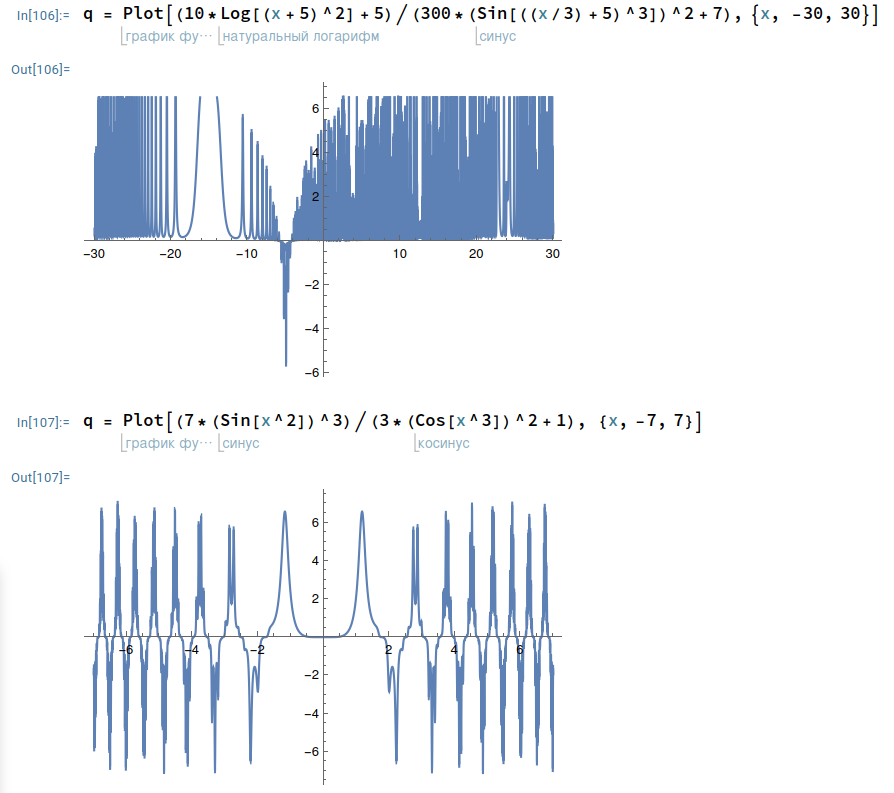
\includegraphics[scale=0.50]{body/img/12_1.png}}
    \label{fig:image_12_1}
\end{figure}